\documentclass[12pt]{article}
\usepackage{mathrsfs}
\usepackage{amssymb}
\usepackage{textcomp}
\usepackage[numbers]{natbib}
\usepackage{float}
\usepackage{CJK}
\usepackage[dvips]{graphics}
\usepackage[sumlimits]{amsmath}
\usepackage{pifont}
\usepackage{bbding}
\usepackage{color}
\usepackage{calrsfs}
\usepackage{bbm}
\usepackage{amssymb}
\usepackage{amsmath}
\usepackage{amsfonts}
\usepackage{url,graphicx,tabularx,array,geometry}
\setlength{\parskip}{1ex} %--skip lines between paragraphs
\setlength{\parindent}{0pt} %--don't indent paragraphs
\setlength{\topmargin}{-20pt}
\setlength{\textheight}{635pt}
\setlength{\textwidth}{430pt}
\setlength{\hoffset}{-20pt}
\setlength{\voffset}{-30pt}
\setlength{\headsep}{10pt}
\makeatletter
\newcommand{\es}[1]{\begin{equation*}\begin{split} #1 \end{split} \end{equation*}}
\newcommand{\rmnum}[1]{\romannumeral #1}
\def\bone{\mathbf{1}}
\def\bY{\mathbf{Y}}
\def\bI{\mathbf{I}}
\def\bU{\mathbf{U}}
\def\bV{\mathbf{V}}
\def\bD{\mathbf{D}}
\def\bE{\mathbf{E}}
\def\bH{\mathbf{H}}
\def\bX{\mathbf{X}}
\def\bR{\mathbf{R}}
\def\bt{\mathbf{t}}
\def\bz{\mathbf{z}}
\def\bx{\mathbf{x}}
\def\logit{\mathrm{logit}}
\def\xii{\mathbf{x}^{(i)}}
\def\tii{\mathbf{t}^{(i)}}
\newcommand{\Rmnum}[1]{\expandafter\@slowromancap\romannumeral #1@}
\makeatother

%-- Commands for header
%\renewcommand{\title}[1]{\textbf{#1}\\}
%\renewcommand{\line}{\begin{tabularx}{\textwidth}{X>{\raggedleft}X}\hline\\\end{tabularx}\\[-0.5cm]}
%\newcommand{\leftright}[2]{\begin{tabularx}{\textwidth}{X>{\raggedleft}X}#1%
%& #2\\\end{tabularx}\\[-0.5cm]}

%\linespread{2} %-- Uncomment for Double Space
\begin{document}

\title{140.756 Final Project\\Simulation Study of Automated Thickness Analyzing Machine (ATAM)}
\author{Chen YUE \& Aaron FISHER} %-- left and right positions in the header
\date{\today}
\maketitle
\begin{abstract}
%In this manuscript, we propose a pipeline for analyzing the relationships between a scalar outcome, and a covariate of the form of a 2D band-shaped structure. Specifically, this method predicts the outcome as a function of the thickness along the length of the 2D structure. Our motivating example is to analyze the link between white matter thickness along the corpus callosum (CC), and Expanded Disability Status Scale (EDSS) score in patients with multiple sclerosis (MS).

In this manuscript we propose a pipeline for analyzing the link between white matter thickness along the corpus callosum (CC) and Expanded Disability Status Scale (EDSS) score in patients with multiple sclerosis (MS). The method can be generally applied to relationships between scalar outcomes and covariates in the form of 2D, band-shaped structures. As this method is still in development, we present here a simulation study applying the method to randomly generated shapes, in order to gauge it's effectiveness.

Our pipeline starts by finding the central curve through each subject's structure, and calculating thickness along the length of the structure based on deviations from this curve. The scalar outcome is regressed on this thickness function and to obtain a fitted coefficient function, which can highlight the portions of the structure that are predicitve of the outcome. Here, we also discuss the creation of pointwise and joint credible intervals for the true coefficient function.

\end{abstract}

\section{Introduction}

Many diseases were found to be related to white matter loss in human brain, such as attention-defict/hyperactivity disorder (ADHD) \cite{Luders2009decreased} and autism \cite{vidal2006mapping}. The change in thickness of the mid-sagittal slice of corpus callosum (CC) was used as a good measurement of the white matter change(loss) in many applications since the CC was the largest white matter structure in human brain and the CC structure could be measured relatively well in magnetic resonance imaging (MRI) or diffusion tensor imaging (DTI) \cite{reich2010automated}. One 3D rendering DTI of CC and its mid-sagittal slice is illustrated in Figure \ref{fig.corpus}. Thus thickness analysis is very important. In this manuscript, we focused on constructing a pipeline of analyzing thickness.\
\begin{figure}[H]
\caption[Corpus callosum data illustration]{\footnotesize Left panel: 3D-rendering of corpus callosum. Right panel: mid-sagittal slice. Views: R=Right, L=Left, S=Superior, I=Interior, A=Anterior, P=Posterior. Produced in 3DSlicer (4.1.1)}
\label{fig.corpus}
\begin{minipage}[b]{0.45\linewidth}
\centering
\scalebox{0.4}{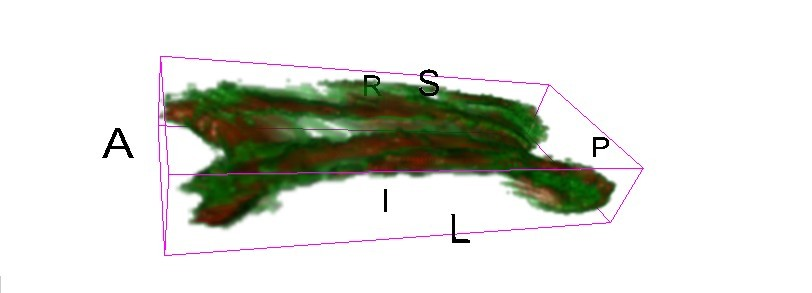
\includegraphics{pics/corpusA5.jpg}}
\end{minipage}
\begin{minipage}[b]{0.45\linewidth}
\scalebox{0.4}[0.3]{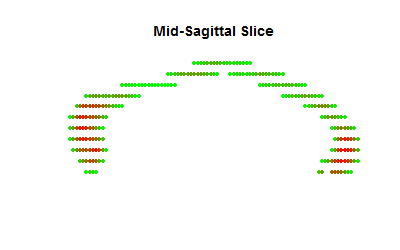
\includegraphics{pics/corpusA3.png}}
\end{minipage}
\end{figure}
Our pipeline had three main steps:
\begin{enumerate}
\item Obtaining center curving and then thickness function along the center curve.
\item Functional regression on a scaler response.
\item Hypothesis testing and figure reconstruction.
\end{enumerate}\

In the first step, principal curve method was implemented. Principal curves \cite{hastie1984principal} are curves that pass through the center of data. The surfaces are fit via nonparametric low-dimensional manifolds that minimize the orthogonal distance from data to themselves. Principal curves satisfy a {\em self consistency} condition, in that they are the conditional expectation (local average) of the data. In another point of view, principal curves minimize the orthogonal distance from the data points to themselves, in contrast to regression and other methods that minimize the distance in one axis. Figure \ref{fig.def} shows the difference between the principal curves and regression. It highlights that the principal curve minimizes the sum of orthogonal distances while a spline model fit tries to minimize the sum of distances parallel to the y axis. Algorithm used in \cite{hastie1989principal} were modified in our work to produce smoothed principal curves. The height functions were achieved using smoothed quantiles of the distances from each data point to the principal curve.\

\begin{figure}[H]
\caption[Principal curves and surfaces]{\footnotesize Left panel is a illustration of different dimension reduction methods. The blue points are the original data points, the dot-dashed green line is the first principal component, the dashed black curve is the spline fitting and the solid red curve is one of the principal curves. Middle panel shows the difference between the principal curve and the regression method: top panel shows that the principal curve minimizes the orthogonal distance, bottom panel shows that the spline regression minimize the distance in y axis. Both panels in the middle use the same dataset. Right panel illustrates several different principal curves for one dataset.}
\label{fig.def}
\begin{minipage}[b]{0.45\linewidth}
\centering
\scalebox{0.37}{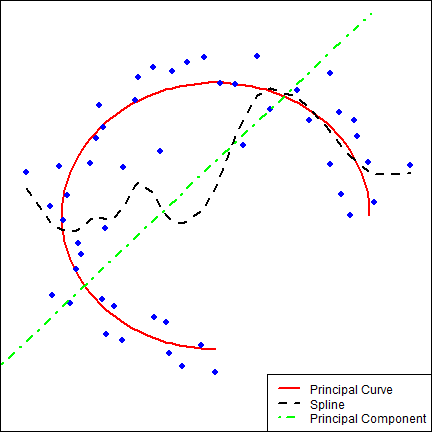
\includegraphics{pics/plot3.png}}
\end{minipage}
\hspace{-1.2cm}
\begin{minipage}[b]{0.45\linewidth}
\centering
\scalebox{0.4}{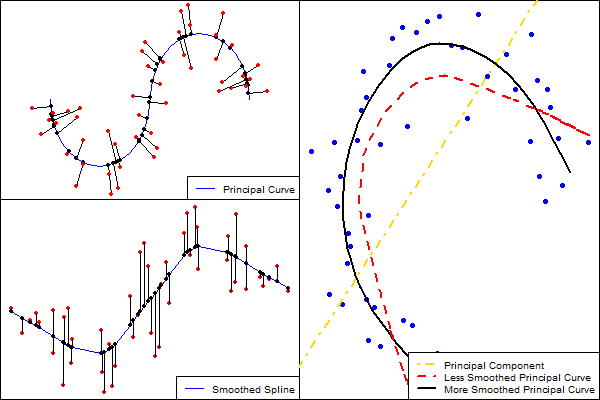
\includegraphics{pics/plot4.png}}
\end{minipage}
\end{figure}

We then regressed our simulated outcome on the height function, using a principle component basis to approximate the hieght function, and a b-spline basis to approximate the coefficent function. Our fitting procedure used a bayesian model, with a priors chosen to impose a roughness penalty on the coefficient function.\cite{goldsmith2010penalized}
\cite{crainiceanu2010bayesian}
\cite{lang2004bayesian}
\cite{Brezger:Kneib:Lang:2005:BaysX}
 Pointwise credible intervals, as well as joint credible intervals, were contructed in a manner similar to that suggested suggested by Crainiceanu, Staicu et. al. (2012).\cite{crainiceanu2012bootstrap}



\section{Simulation Settings}
In current work, two cases of simulations were proposed. The number of individuals (images and responses) are 300 in both cases. The scale response in both cases were 300 random numbers generated from a poisson distribution with mean 3, denoted as $Y_i,\ i=1,\dots,I=300$.
\subsection{Case 1: letter ``C"}
Let $\theta_{n}\sim \text{Unif}(\frac{\pi}{3},\frac{7\pi}{4})$, $\delta_n\sim \text{Unif}(0.1,0.3)$ and $r_{n}\sim \text{Unif}(1-\text{thick}_n, 1+\text{thick}_n)$ , where $n=1,\dots,N=500$:
\begin{equation*}
\text{thick}_n=\left\{\begin{array}{ll}\frac{2}{5}\log(Y_i+1)& \theta_n\le \frac{3\pi}{4}\\ \delta_n & \theta_n\in (\frac{3\pi}{4},\frac{5\pi}{4}]\\\frac{1}{5}\log(Y_i+1)&\theta_n\in [\frac{5\pi}{4},\frac{7\pi}{4})\end{array}\right..
\end{equation*}
Then we let $z_{n1}=r_n\sin\theta_n$ and $z_{n2}=r_n\cos\theta_n$. Six of the three hundred images are illustrated in Figure \ref{fig.Cshape}. This figure shows how the thickness of top and bottom parts of the letter ``C" are determined by the scaler response $Y_i$ while the thickness of the middle part was determined by a totally independent random variable $\delta$. \

\begin{figure}[H]
\caption[``C"-shape data cloud]{\footnotesize Simulated ``C"-shape data cloud}
\label{fig.Cshape}
\begin{minipage}[b]{1\linewidth}
\centering
\scalebox{0.35}{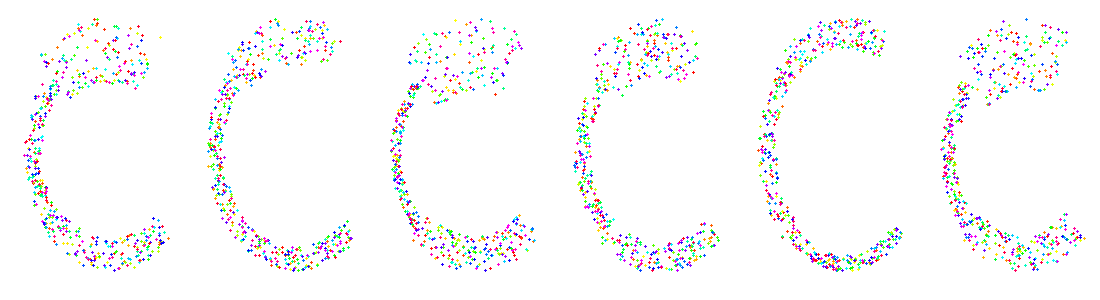
\includegraphics{pics/Simulation_C.png}}
\end{minipage}
\end{figure}\

\subsection{Case 2: digit ``5"}
Three hundred images generated in the general shape of the number ``five''. Six examples of these shapes are illustrated in Figure \ref{fig.fiveshape}. The thickness of the vertical bars on top was set to vary with the response $Y_i$, while other parts of the ``five" yielded thickness control by a independent variable $\delta$.\

Specifically, let $z_{n1}\sim U(0,1)$, $z_{n2}=\epsilon_n$ when $n=1\dots,3N/10$; $z_{n1}=\epsilon_n$, $z_{n2}\sim U(-1,0)$ when $i=3N/10+1,\dots,4.5N/10$; $z_{n1}\sim U(0,0.5)$, $z_{n2}=-1+\epsilon_i$ when $i=4.5N/10+1,\dots,6N/10$; $z_{n1}=\frac{1}{2}+(\frac{1}{2}+\epsilon_n)\cos(\theta_n)$, $z_{n2}=-\frac{3}{2}+(\frac{1}{2}+\epsilon_n)\sin(\theta_n)$ for $i=6N/10+1,\dots,8.5N/10$ where $\theta_n\sim U(-\pi/2,\pi/2)$; $z_{n1}\sim U(0,0.5)$, $z_{n2}=-2+\epsilon_n$ when $n=8.5N/10+1,\dots,N$. N was chosen to be 3,000 and $\delta_i\sim \text{Unif}(0.03,\ 0.10)$ and $\epsilon_n\sim N(0, \delta_i)$ when $n\notin \{3N/10+1,\dots,4.5N/10\}$ and let $\epsilon_n\sim \text{Unif}(-Y_i/20,Y_i/20)$ when $n\notin \{3N/10+1,\dots,4.5N/10\}$.\


\begin{figure}[H]
\caption[``5"-shape data cloud]{\footnotesize Simulated ``5"-shape data cloud}
\label{fig.fiveshape}
\begin{minipage}[b]{1\linewidth}
\centering
\scalebox{0.35}{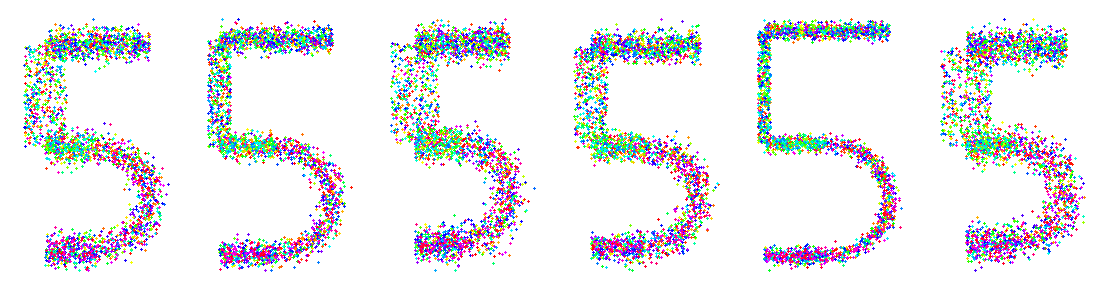
\includegraphics{pics/Simulation_5.png}}
\end{minipage}
\end{figure}\

\section{Principal Curves and Thickness Function}
In this whole pipeline, the first step would be calculating the center curves of the data cloud. The method we were using was called the principal curves \cite{hastie1989principal}.
\subsection{Principal Surfaces}
Let $\mathbf{x}_i=(x_{i1},x_{i2})^T,\ i=1,\dots, I$ be the data points in two dimensional space, $\mathcal{R}^2$, $t_i$ be corresponding parametrization points in real line, $\mathcal{R}$. In addition, we will require (without loss of generality) that the coordinate $t_i$ ranging from 0 to 1. We define $f$ as the smooth principal curve function $f: t_i\mapsto f(t_i)$ that maps from $\mathcal{R}$ to $\mathcal{R}^2$. The principal curve function satisfies the {\em self-consistency} condition:
\begin{equation}
E(\bX|\lambda_f(\bX)=\bt)=f(\bt)\ \ \text{for all }\bt,
\end{equation}
where $\lambda_f(\bx)=\sup_{\mathbf{t}}\big\{\mathbf{t}: \|\mathbf{x}-f(\mathbf{t})\|=\inf_{\mathbf{\mu}}\|\mathbf{x}-f(\mathbf{\mu})\| \big\}$ is the projection function with respect to $f$. The projection function maps a data point on to the closest principal curve point having the largest parametrization.
\citeauthor{hastie1989principal} \cite{hastie1989principal} showed that principal curves generally exist, though are not unique. We have found that there are two main distinctions between different fitted principal curves: the degree of smoothness and the method of parametrization. In most algorithms, these properties will be controlled by the specific smoother being used in the algorithm and its tuning parameters. The details of our specific algorithm will be demonstrated in the next section.\

\subsection{Algorithm}
In this paper, the algorithm used in \cite{hastie1989principal} will be modified. This algorithm allows us to find the curves coordinate for each data point ($\mathbf{t}_i, i=1,\dots, I$), which we will use later to create parametric summaries. However, the original principal curve algorithm can only yield surfaces which are locally flattened. Therefore, instead of local planar smoothers, we employ thin-plate spline (TPS) for fitting the surface. Thin-plate splines were proposed by \cite{duchon1977splines} and are now widely used for single variate or bivariate smoothing. The TPS penalize the least squares error by a high-order derivative term in order to achieve a desired degree of smoothness. \citeauthor{wood2003thin} \cite{wood2003thin} improved the computational efficiency when fitting TPS by using an optimal approximating basis that we employ.\

{\bf Preprocessing.} Recall the notation we defined in section 2.2, let $\mathbf{X}=[\mathbf{x}_1, \dots, \mathbf{x}_I]^T$ be the $I\times 2$ matrix that contains the 2D coordinates of the dataset. We assumed that the data are demeaned and centered around the origin. Principal component decomposition is then applied. Let $\mathbf{X}=\mathbf{U}\mathbf{\Sigma}\mathbf{V}^T$ be the singular value decomposition of $\mathbf{X}$. Then $\mathbf{U}\tilde{\mathbf{\Sigma}}$ are the first principal ``scores" of the data matrix, where $\tilde{\mathbf{\Sigma}}$ is a submatrix of $\mathbf{\Sigma}$ containing only the first column. We then standardized the scores so that they are in $[0,\ 1]$, and use them as the initial parametrization of $\mathbf{x}_i$.\

{\bf Conditional Expectation.} Suppose $t_i$ be the current parametrization of $\mathbf{x}_i$ in $[0,1]$. For a specific data point $\bx_0$, with its coordinate $t_0$, we choose $r$ as a radius, such that all the other data points with their projection coordinate having less distance from $\bt$ than $r$ are considered as the neighbor of $\bx$, see the left panel in Figure \ref{fig.alg}. Let $\mathcal{N}_{\bx_0}$ be the set of all the neighbors of the point $\bx_0$. Then we have $\mathcal{N}_{\bx_0}=\big\{\bx_j :\ \|\bt_{j}-\bt_0\|\le r \big\}$ and we calculate the local average $\bx^{lm}=\text{Avg.}\{\bx_j:\ j \in\mathcal{N}_{\bx_0}\}$.

{\bf Smoothing.} Thin plate splines \cite{wood2003thin} are applied after we obtained these local averages: $\bx_i^{lm},\ i=1,\dots,I$. In this step, we fitted
\begin{equation}
x^{lm}_{id}=f_{d}(t_{i})+\epsilon_{id},\ \ d=1,2,
\end{equation}
and obtained a thin plate spline smoothing of the local average points, which is demonstrated in the right panel of Figure \ref{fig.alg}.

\begin{figure}[H]
\caption[Principal surfaces algorithm]{\footnotesize Left panel illustrates the projection step and the conditional expectation step, right panel illustrates the smoothing step}
\label{fig.alg}
\begin{minipage}[b]{0.45\linewidth}
\centering
\scalebox{0.7}{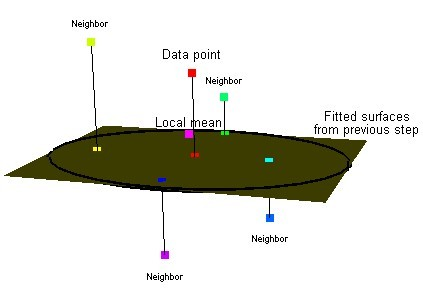
\includegraphics{pics/alg_1.jpg}}
\end{minipage}
\hspace{1cm}
\begin{minipage}[b]{0.45\linewidth}
\centering
\scalebox{0.6}{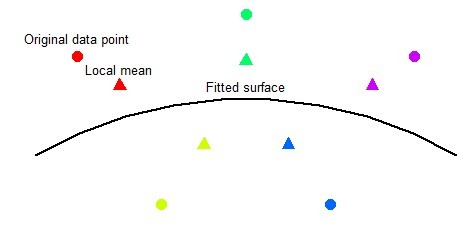
\includegraphics{pics/alg_2.jpg}}
\end{minipage}
\end{figure}

{\bf Projection.} We then projected each data point onto the current principal curve and obtain new 2D parametrization. Notice that we used grid search method to find the projection and we only search within the range $[0,1]$. Therefore there will be some data points being projected onto the boundary which brings some issues when we further analyzed the parametrization. After this step, we iterate the whole procedure with the new parametrization $t_{i+1}$, and repeate the process until we get convergence of the $t_i$ terms.\

\subsection{Fitting Result of Principal Curves}
The principal curve fitting results are illustrated in Figure \ref{fig.PS}. Starting with the upper panel in Figure \ref{fig.PS}, one can see the algorithm reconstruct the ``C" shape data cloud quite well. Due to the large thickness on the top part of ``C", there are issues that the algorithm bend the curve back toward inside (in the first panel on the left). However, for most of the cases, the results are satisfactory. The ``5" reconstructions are illustrated in the bottom panels. Most of the fitted are recovered well for all cases.\

\begin{figure}[H]
\caption[Principal Curves]{\footnotesize Principal curves fitting results. top panels illustrate the results for ``C"-shape data; bottom panels shows the results for ``5"-shape data.}
\label{fig.PS}
\begin{minipage}[b]{1\linewidth}
\centering
\scalebox{0.35}{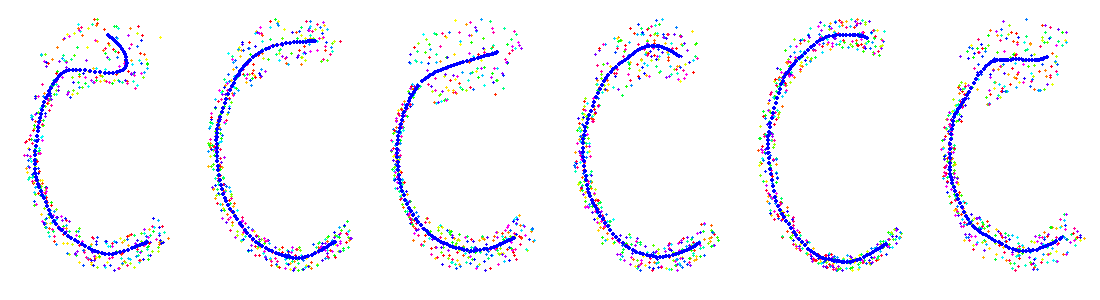
\includegraphics{pics/PCurve_C.png}}
\vspace{-0.3cm}
\scalebox{0.35}{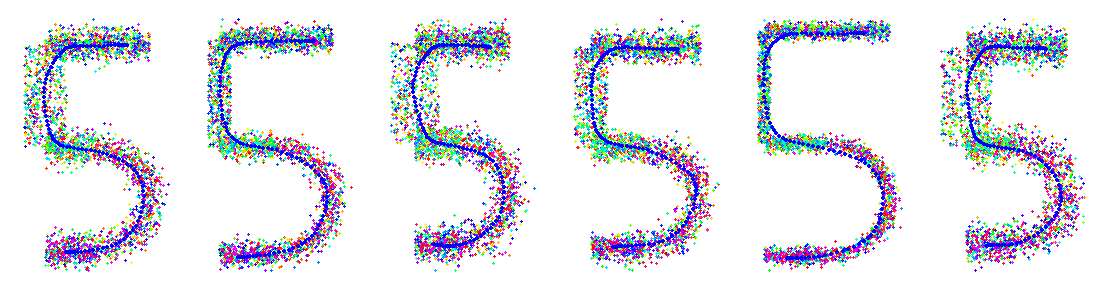
\includegraphics{pics/PCurve_5.png}}
\end{minipage}
\end{figure}\

\subsection{Obtaining Thickness Functions}
Constructing the thickness functions along principal curves then followed, which is shown in Figure \ref{fig.thick}. We first calculated the distances from all data points to their projections on the curve. Second, we used two times the $95\%$ quantile of all the distances within a window around a center, $t_0$ as the raw height at $t_0$ on the curve. Last, we smoothed those raw height using smoothed splines. The result showed clear patterns of which part the image yielded varied thickness. These information would be further analyzed using functional regression on scaler.

\begin{figure}[H]
\caption[Smoothed Thickness Function]{\footnotesize Smoothed thickness functions. Left panel illustrates thickness function for ``C"-shape data and right panel shows the ones for ``5"-shape data.}
\label{fig.thick}
\begin{minipage}[b]{0.5\linewidth}
\centering
\scalebox{0.33}{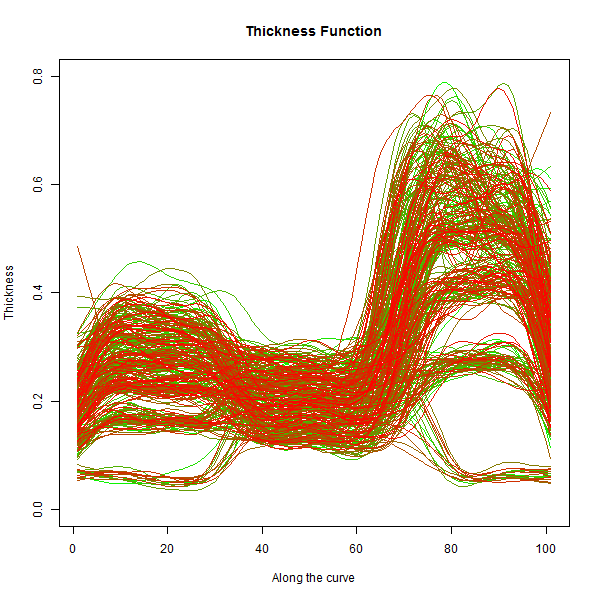
\includegraphics{pics/thickness.png}}
\end{minipage}
\hspace{0.2cm}
\begin{minipage}[b]{0.5\linewidth}
\centering
\scalebox{0.33}{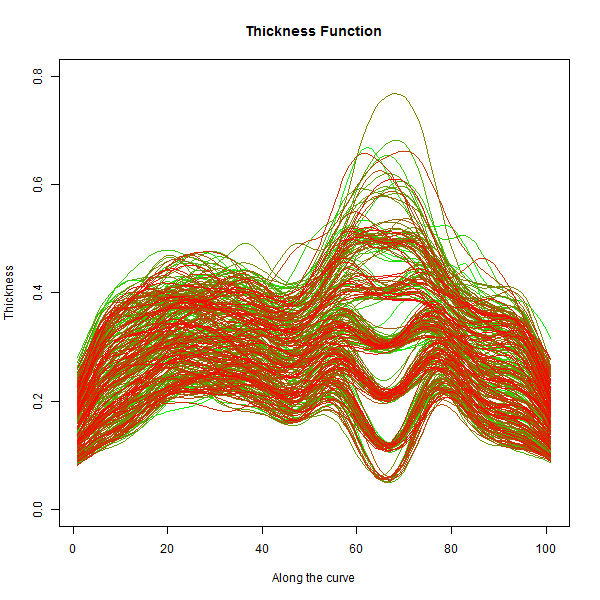
\includegraphics{pics/thickness2.png}}
\end{minipage}
\end{figure}
\section{Functional Regression}
Once thickness functions for each simulated subject were obtained, we used Bayesian machenery to regress the simulated outcome $Y_i(t)$ against the thickness curve. Let $X_i(t)$ denote the value of the thickness function at location $t$, with $t$ varying from $0$ to 1. We model $Y$ as a poisson random variable, with $log(E(Y_i)) = \beta_0+ \int_0^1 X_i(t)\beta(t)dt$. In order to carry out the regression, we express $X_i(t)$ as a linear combination of it's first 35 principle components, and approximate $\beta(t)$ using 35 equally spaced b-splines. This number of basis functions was chosen based on the general suggestion of Goldsmith et. al. (2010). \cite{goldsmith2010penalized}. Thus, we approximate $\int_0^1 X_i(t)\beta(t)dt$ as:

\es{
\int_0^1 X_i(t)\beta(t) dt & \approx \int_0^1 \left( \sum_{k\in \{A\} } \xi_{ik} \Psi_k(t) \right) \left( \sum_{ j\in \{ B\}} \beta_j \varphi_j(t)  \right)dt   \\
}
Where $\Psi_k(t)$ is the $k^{th}$ principle component of $X(t)$, $\xi_{ik}$ is the $i^{th}$ subject's score for the $\Psi_k(t)$, $\varphi_j(t)$ is the $j^{th}$ b-spline for $\beta(t)$, $\beta_j$ is the coefficient for $\varphi_j(t)$, and the sets $\{A\}$ and $\{B\}$ are both equal to $\{1,2,... 35 \}$. Now we can represent $\int_0^1 X_i(t)\beta(t)$ as a design matrix by noting that:

\es{
 \approx \int_0^1 \left( \sum_{k\in \{A\} } \xi_{ik} \Psi_k(t) \right) \left( \sum_{ j\in \{ B\}} \beta_j \varphi_j(t)  \right)dt    &=\int_0^1 \left(  \sum_{(k,j)\in \{A\}\times \{B\} } \xi_{ik} \Psi_k(t)    \varphi_j(t)   \beta_j \right) dt \\
 &=  \sum_{(k,j)\in \{A\}\times \{B\} } \xi_{ik}  \left( \int_0^1 \Psi_k(t)    \varphi_j(t)  dt \right) \beta_j  \\
 &=: \xi_{i} \bold{J} \beta^T  \\
 }

Where $\xi_i=[\xi_{i1},..\xi_{i35}]^T$, $\beta=[\beta_1,...\beta_{35}]^T$, and $\bold{J}$ is a $35 \times K_\beta$ matrix with $(i,j)^{th}$ element equal to $ \int_0^1 \Psi_i(t)    \varphi_j(t) dt$. The elemnts of $\bold{J}$ can be approximated numerically. \cite{goldsmith2010penalized} \cite{crainiceanu2010bayesian}

For this project we assume $\xi_{i} \bold{J}$ is a fixed element of our design matrix. In order to enforce smoothness on our fitted $\beta(t)$, we apply a first-order random walk prior on $\beta_j$ coefficients, such that $\beta_j$ is assumed apriori to be is normally distributed around $\beta_{j-1}$. Because our bases is a b-spline basis, this will cause induce continuity in $\beta(t)$ by encouraging position-dependent autocorrelation.\cite{crainiceanu2010bayesian}
\cite{lang2004bayesian}
\cite{Brezger:Kneib:Lang:2005:BaysX}

Our final regression model is:\footnote{One extension of this model would be to account for measurement error by letting: $W_i(t)=
\sum_{k=1}^{K_x} \xi_{ik} \Psi_k(t) + \epsilon_i(t)$, and assigning priors for $\epsilon_i(t)$ and $\xi_{ik}$.\cite{crainiceanu2010bayesian} Again tough, we have not incorporated this into our model at this point in time.}

\es{
Y_i \sim Poisson(\theta_i) \\
 \theta_i  = \beta_0+ \xi_{i} \bold{J} \beta^T  \\
\beta_0, \beta_1 \sim N(0,100) \\
 \beta_j \sim N(\beta_{j-1},1/\tau_\beta) \\
 \tau_\beta \sim \Gamma(.001,.001)\\
 }


We fit our regression using an MCMC in WinBUGS, with a burn in period of 100,000. All parameters appeared to mix well through a target distribution, with the notable exception of $\tau_\beta$, which showed a high variability. Still, our reconstructed $\beta(t)$ estimates were fairly stable. We discuss these results and their interpretation in more detail in section 5.

\section{Hypothesis Testing}

Let $d$ denote the index of a draw from our posterior distribution of parameters. In order to get the posterior distribution of the $\beta(t)$, we can reconstruct a $\beta_d(t)$, for each draw $d$, from our posterior distributions for $\{\beta_1,\beta_2, ... \beta_{35}\}$ using our b-spine bases. Let $\hat{\beta}(t) := mean(\beta_d(t))$ be our estimate of the true $\beta(t)$.

We are interested in finding credible pointwise intervals for $\beta(t)$ and joint credible intervals for $\beta(t)$, such that 95\% of the $\beta_d(t)$ values lie within the 95\% pointwise credible interval band at any position $t$, and 95\% of the $\beta_d(t)$ curves are completely contained within the 95\% joint credible interval bands around $\hat{\beta}(t)$. Because we have a posterior distribution for $\beta(t)$, we can calcuate both intervals directly.

To get an estimate for the 95\% pointwise interval, we can simply take the .025 and .975 quantiles of $\beta_d(t)$ at each point $t$ in our curve.

In order to get the 95\% joint credible interval, we use a method similar to one outlined by Crainiceanu et. al. (2012).\cite{crainiceanu2012bootstrap} First we make the assumption that the for any constant $k$, the probability that $\beta_d(t)$ is at least $k$ standard deviations away from $\hat{\beta}(t)$ is constant accross $t$. Roughly speaking, this assumption leads to the intuition that if we want to find the bound that completely contains 95\% of all $\beta_d(t)$ curves, we should let this bound be proportional to the standard deviation of $\beta_d(t)$ as a function of $t$. If we can get the distribution for farthest distance each curve gets from $\hat{\beta}(t)$, in units of standard deviation, then the 95\% quantile of this distribution will denote the mark that 95\% of these curves never surpass.

More specifically, to get the joint credible intervals, let $\sigma(t)^2 = var(\beta_d(t))$, $S_d(t) = \frac{|\beta_d(t)-\hat{\beta}(t)    | } {\sigma(t)}$, and let $m_d= max_t \left\lbrace S_d(t) \right\rbrace$. Then, if $q(m_d,.95)$ is the 95\% quantile of $m_d$ across $d$, then we can reconstruct credible bands using $\hat{\beta}(t) \pm  q(m_d,.95)\sigma(t)$.\footnote{As an intermediate step, note that if we  if we scale the $\beta_d(t)$ cruves to have standard deviation equal to 1 accross their entire length (i.e. for all $t$), then $\hat{\beta}(t) \pm q(m_d,.95)$ is a joint credible interval for the resulting scaled curves.}

As a comparison, we can also construct a Bonferroni based joint confidence interval based on the formula for the pointwise interval. Note that we approximated the interval for $t$ with a grid of 101 points, so if $q(\beta_d(t), .p)$ is the $p^{th}$ quantile of $\beta_d(t)$ at time $t$, then a highly conservative joint interval can be found by using the pointwise ($\alpha$/101) and (1-$\alpha/101$) quantiles. A comparison of this method against the joint band method described above is shown in Figure \ref{fig.bands}. 

\begin{figure}[h!]
\caption[]{\footnotesize On the left we show the credible intervals for the ``five'' shaped data. Intervals for ``C" shaped data are shown on the right. For the ``C" data, the true $beta(t)$ is highest at the end segments of the curve. For the ``5" data, the true $\beta(t)$ is highest around the indexes 60-80. Estimates of $\beta(t)$ are shown in solid black, pointwise intervals are shown as dotted black lines, joint credible intervals calculated using the distribution of $m_d$are shown as dotted red lines, and bonferroni joint credible intervals are shown as dotted blue lines.}
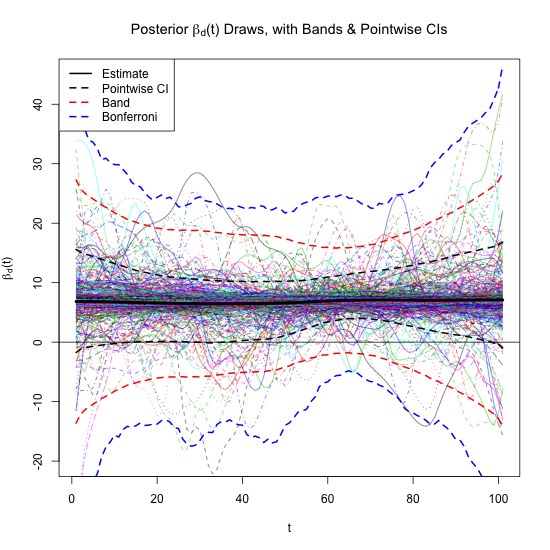
\includegraphics[scale=.45]{pics/Figure_Bands_5_Shape_12-19-12_bonf.png} 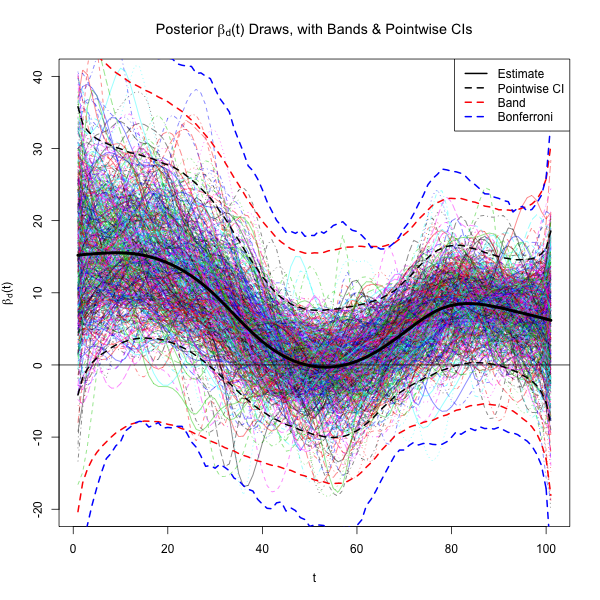
\includegraphics[scale=.41]{pics/Figure_Bands_C_Shape_12-19-12_bonf.png}
\label{fig.bands}
\end{figure}

As Figure \ref{fig.bands} shows, the joint credible interval includes zero accross the entire domain of the function, so we can't say that any point is clearly significant without further testing. However, several of the points corresponding to areas where the true $\beta(t)$ is positive are pointwise significant, where as most areas where the true $\beta(t)$ function is zero are not pointwise significant. Thus, at this stage of our method's development, the pipeline seems appropriate for generating hypothesis about where to look for the true $\beta(t)$, but it is not sufficiently powerful to find these points to be immediately significant.

In Figure \ref{fig.final}, we show six examples of mapping these results back onto the original shapes. Different color along the principal curves indicates the magnitude of the quantity $\hat{\beta}(t)\Big/(\frac{1}{2}W_{CI}(t))$, where $W_{CI}(t)$ is the 95\% width of the credible interval at coordinate $t$. In both case, the quantities are compared with the value 1 if pointwise 95\% confidence level is used, but higher value indicates stronger evidence that the thickness is related to the scaler outcome. The back mapping procedure discovers the thickness-response related regions successfully. However, hard threshold at 1 was not satisfactory in both cases due to the fixed pointwise confidence level might depend on cases and even locations along the curve.

\begin{figure}[H]
\caption[Back-mapping]{\footnotesize Upper figures illustrate the back mapping result for case ``C", bottom figures shows the result for case ``5". Color along the principal curves indicate the magnitude of the quantity $\hat{\beta}(t)\Big/(\frac{1}{2}W_{CI}(t))$, where $W_{CI}(t)$ is the width of the credible interval at coordinate $t$.}
\label{fig.final}
\begin{minipage}[b]{1\linewidth}
\centering
\scalebox{0.35}{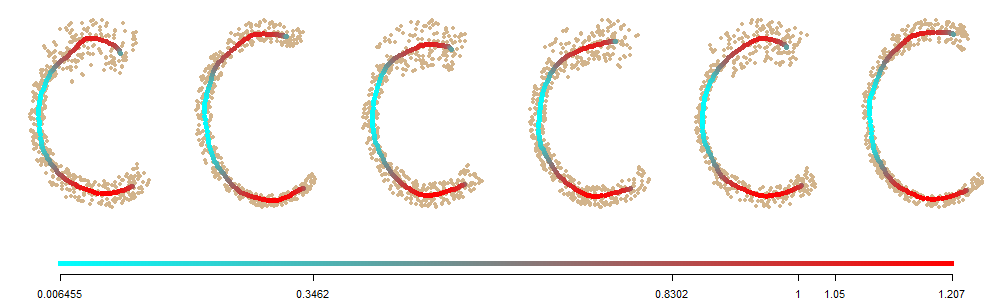
\includegraphics{pics/final_C.png}}
\scalebox{0.35}{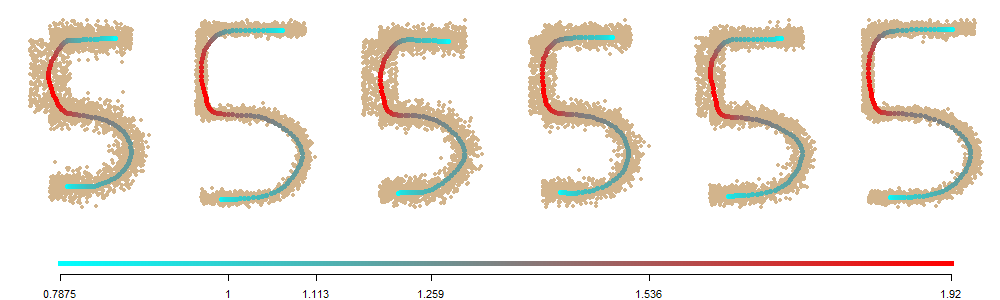
\includegraphics{pics/final_five.png}}
\end{minipage}
\end{figure}\

\section{Discussion}

We propose a method to find the thickness of a structure across it's length, and to regress this thickness function against a scalar outcome. The results of a simulation study for this method show that it is generally capable of identifying the true signal regions as pointwise significant, but not yet capable of identifything them as jointly significant.

With regard to the nature of the simulated data, it is possible that we were aided by the fact that there was not much signal in the simulated $X(t)$ curves beyond the signal that was related to $Y$. Thus, the first principle component of the data explained almost all of the variation of $X(t)$, and, in general, the principle component basis gave a good approximation. However, a feature of the simulated dataset that likely worked against us was that the true $\beta(t)$ function had noncontinuous jumps. Our method assumes a continuous and fairly smooth underlying $\beta(t)$, and although it did reasonably well on estimating our simulated $\beta(t)$, it may do better on data where the true underlying $\beta(t)$ is smooth.

Some problems we encountered included the issue that our priciple curve fitting method struggled to accurately fit the tail ends of a structure, especially when the structure had fat tails. We also had to choose a number of principle components and b-splines to use, and our were results were slightly sensitive to this choice.




\bibliographystyle{plainnat}
\nocite{*}
\bibliography{thickcite}

\end{document}
